% ══════════════════════════════════════════════════════════════════════════════
% Earthquake Magnitude Estimation Using Ensemble Machine Learning
% Journal-Standard LaTeX (IEEE Transactions Style)
% ══════════════════════════════════════════════════════════════════════════════
\documentclass[journal,10pt,twocolumn]{IEEEtran}

% ── Packages ─────────────────────────────────────────────────────────────────
\usepackage[utf8]{inputenc}
\usepackage[T1]{fontenc}
\usepackage{amsmath,amssymb,amsfonts}
\usepackage{graphicx}
\usepackage{booktabs}
\usepackage{multirow}
\usepackage{hyperref}
\usepackage{xcolor}
\usepackage{float}
\usepackage{algorithm}
\usepackage{algorithmic}
\usepackage{cite}
\usepackage{balance}
\usepackage{microtype}
\usepackage{url}
\usepackage{array}
\usepackage{tabularx}
\usepackage{caption}
\usepackage{subcaption}

% ── Graphics path ────────────────────────────────────────────────────────────
\graphicspath{{figures/}}

% ── Hyperref setup ───────────────────────────────────────────────────────────
\hypersetup{
    colorlinks=true,
    linkcolor=blue!70!black,
    citecolor=green!50!black,
    urlcolor=blue!60!black
}

% ══════════════════════════════════════════════════════════════════════════════
\begin{document}

\title{Earthquake Magnitude Estimation Using Ensemble\\Machine Learning with Engineered Spatiotemporal Features}

\author{
    \IEEEauthorblockN{Arijit Mondal}
    \IEEEauthorblockA{
        Department of Computer Science\\
        \textit{Independent Research}\\
        Email: ariktheone@github
    }
}

\maketitle

% ══════════════════════════════════════════════════════════════════════════════
\begin{abstract}
Earthquake magnitude estimation from pre-event seismological parameters remains a fundamental challenge in computational seismology. This study presents a comprehensive machine learning pipeline that evaluates 11 regression algorithms on 18,030 California earthquakes recorded by the Northern California Seismic Network (NCSN) from 1966 to 2007. We engineer 59 features spanning five categories—temporal, spatial, seismological, rolling/lag statistics, and encoded categorical variables—and evaluate models including linear methods, tree-based ensembles, gradient boosting, and XGBoost. After initial screening, the top three models undergo hyperparameter optimization via randomized cross-validated search. The tuned Extra Trees Regressor achieves the best performance with $R^2 = 0.3297$, MAE $= 0.2522$, RMSE $= 0.3463$, and MAPE $= 7.12\%$ on a held-out 30\% test set. We analyze feature importance, finding that the number of recording stations (11.98\%), magnitude type encoding (8.66\%), and temporal features collectively contribute most to predictive power. While the moderate $R^2$ reflects the inherent stochasticity of earthquake magnitudes, the sub-0.26 MAE demonstrates practical utility for relative magnitude estimation within a well-instrumented network. The complete pipeline, trained model, and interactive Streamlit visualization tool are released as open-source software.
\end{abstract}

\begin{IEEEkeywords}
earthquake magnitude estimation, ensemble learning, Extra Trees, feature engineering, seismology, machine learning, spatiotemporal features
\end{IEEEkeywords}

% ══════════════════════════════════════════════════════════════════════════════
\section{Introduction}
\label{sec:introduction}

Earthquakes constitute one of the most destructive natural hazards, causing significant loss of life and economic damage worldwide. The deterministic prediction of earthquake occurrence—specifying the time, location, and magnitude of future events—remains scientifically elusive \cite{geller1997}. However, the \emph{estimation} of earthquake magnitudes from measurable seismological parameters represents a more tractable problem with practical applications in seismic hazard assessment and early warning systems.

Traditional magnitude estimation relies on empirical relations derived from waveform analysis \cite{kanamori1977}. With the proliferation of dense seismic networks and digital recording infrastructure, machine learning (ML) approaches have shown promise in supplementing these classical methods by exploiting high-dimensional feature spaces that encompass spatial, temporal, and instrumental parameters \cite{mousavi2020, derakhshani2013}.

This study contributes:
\begin{enumerate}
    \item A systematic comparison of 11 regression algorithms for magnitude estimation using NCSN catalog data;
    \item An engineered feature set of 59 variables derived from 13 raw catalog columns, with explicit leakage prevention in lag and rolling computations;
    \item Hyperparameter optimization of the top-performing models via randomized cross-validated search;
    \item A fully reproducible, open-source pipeline integrated with an interactive Streamlit dashboard for visualization and benchmarking.
\end{enumerate}

The remainder of this paper is organized as follows: Section~\ref{sec:related} surveys related work. Section~\ref{sec:data} describes the dataset. Section~\ref{sec:methodology} details feature engineering and modeling methodology. Section~\ref{sec:results} presents experimental results. Section~\ref{sec:discussion} discusses findings and limitations. Section~\ref{sec:conclusion} concludes.

% ══════════════════════════════════════════════════════════════════════════════
\section{Related Work}
\label{sec:related}

Machine learning applications in seismology have grown substantially over the past decade. \textbf{Magnitude estimation} approaches span from early neural network studies \cite{mousavi2020} to modern deep learning architectures trained on waveform data \cite{perol2018}. Catalog-based studies, which use event metadata rather than raw waveforms, have employed random forests \cite{derakhshani2013}, support vector machines, and gradient boosting machines with varying degrees of success.

\textbf{Feature engineering} for seismic applications typically includes spatial coordinates, depth, recording network parameters (station count, azimuthal gap), and temporal features \cite{asim2018}. Rolling and lag statistics captured from event sequences have been explored in aftershock prediction but are less commonly applied to magnitude estimation.

\textbf{Ensemble methods}—Random Forest, Gradient Boosting, Extra Trees, and XGBoost—have consistently outperformed linear and single-tree models in geophysical applications due to their ability to capture nonlinear relationships and interaction effects \cite{bergen2019}.

This work differentiates itself by: (a) evaluating a broader set of 11 algorithms under uniform conditions, (b) systematically engineering 59 features with rigorous leakage prevention, and (c) providing a complete, reproducible pipeline with interactive visualization.

% ══════════════════════════════════════════════════════════════════════════════
\section{Dataset}
\label{sec:data}

\subsection{Source and Scope}

We use the Northern California Seismic Network (NCSN) earthquake catalog, comprising 18,030 events recorded between 1966 and 2007 in California, USA. The catalog is curated from the Northern California Earthquake Data Center (NCEDC) \cite{ncedc}.

\subsection{Raw Features}

Table~\ref{tab:raw_features} summarizes the 13 columns in the processed dataset.

\begin{table}[!t]
\centering
\caption{Raw Dataset Schema (13 Columns)}
\label{tab:raw_features}
\begin{tabular}{@{}lll@{}}
\toprule
\textbf{Column} & \textbf{Type} & \textbf{Description} \\
\midrule
Date & datetime & Event date (YYYY/MM/DD) \\
Time(UTC) & datetime & Event time \\
Latitude & float & Epicenter latitude (°) \\
Longitude & float & Epicenter longitude (°) \\
Depth(km) & float & Hypocentral depth \\
Magnitude & float & \textbf{Target} (3.0–7.39) \\
Mag\_type & categorical & Magnitude scale type \\
No\_of\_Stations & int & Recording stations \\
Gap & float & Azimuthal gap (°) \\
Close & float & Nearest station dist. \\
RMS & float & Travel-time residual \\
SRC & categorical & Source network (NCSN) \\
EventID & int & Unique identifier \\
\bottomrule
\end{tabular}
\end{table}

\subsection{Descriptive Statistics}

The magnitude distribution (Fig.~\ref{fig:mag_dist}) is right-skewed with a mean of 3.43 and standard deviation of 0.42. The majority of events (>90\%) have magnitudes below 4.0, reflecting the Gutenberg-Richter frequency-magnitude relationship. The spatial distribution (Fig.~\ref{fig:spatial_dist}) reveals clustering along known California fault systems, particularly the San Andreas Fault and its subsidiaries.

\begin{figure}[!t]
\centering
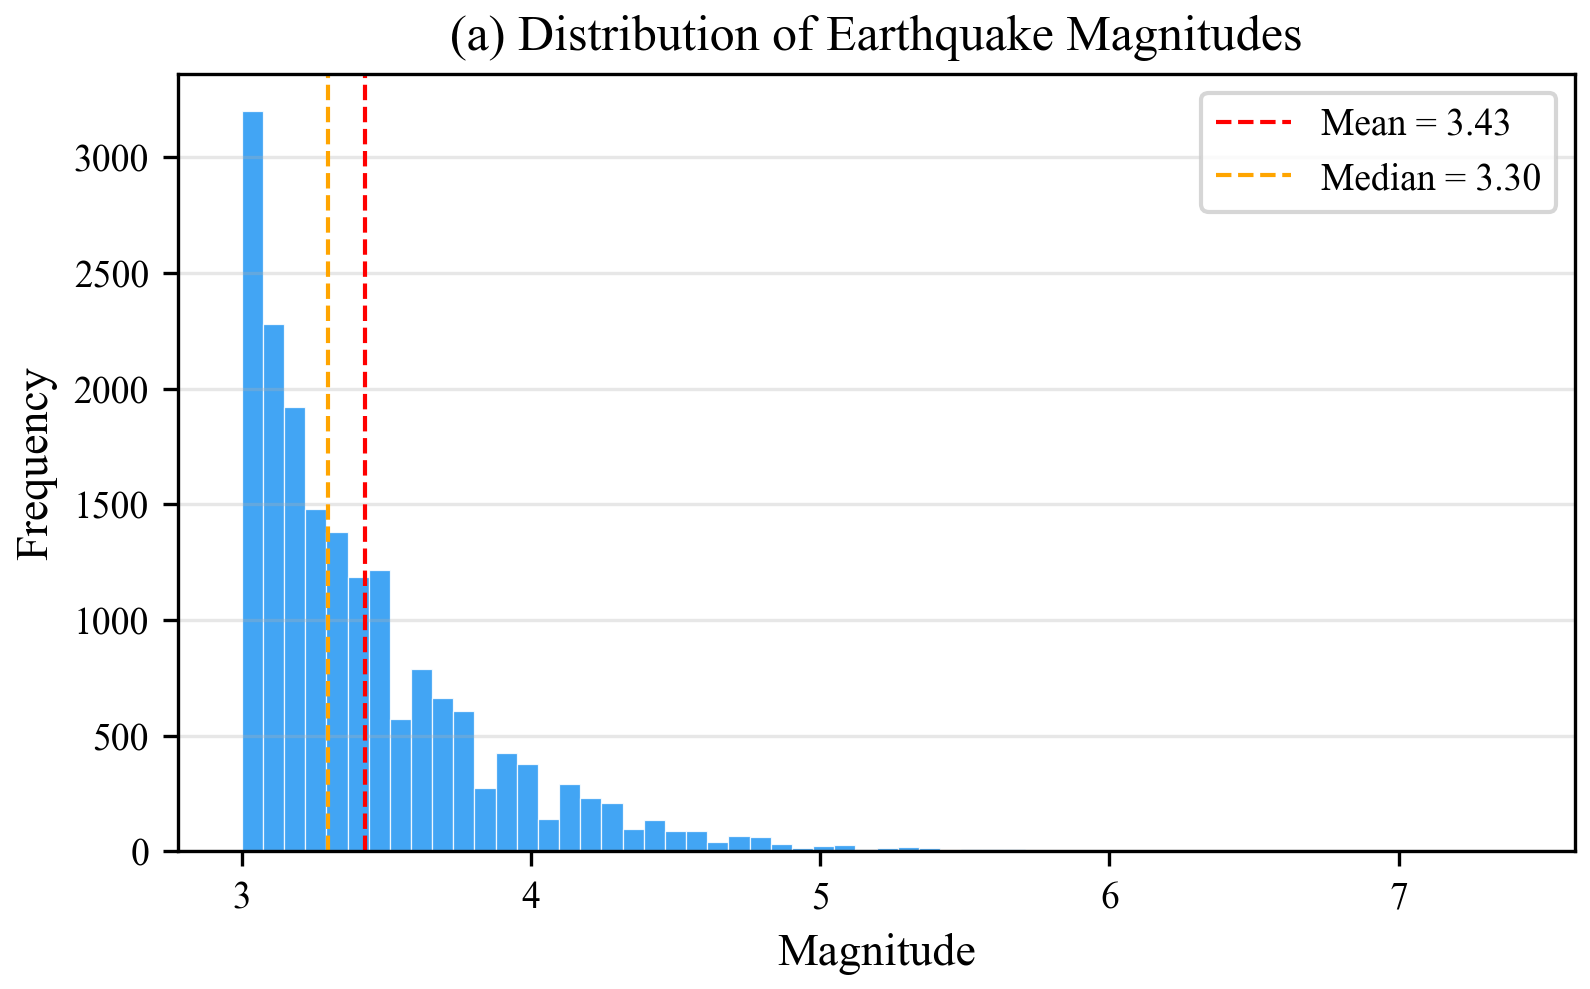
\includegraphics[width=\columnwidth]{fig1_magnitude_distribution.png}
\caption{Distribution of earthquake magnitudes in the NCSN catalog (1966–2007). The distribution follows the expected Gutenberg-Richter power law with $b \approx 1$.}
\label{fig:mag_dist}
\end{figure}

\begin{figure}[!t]
\centering
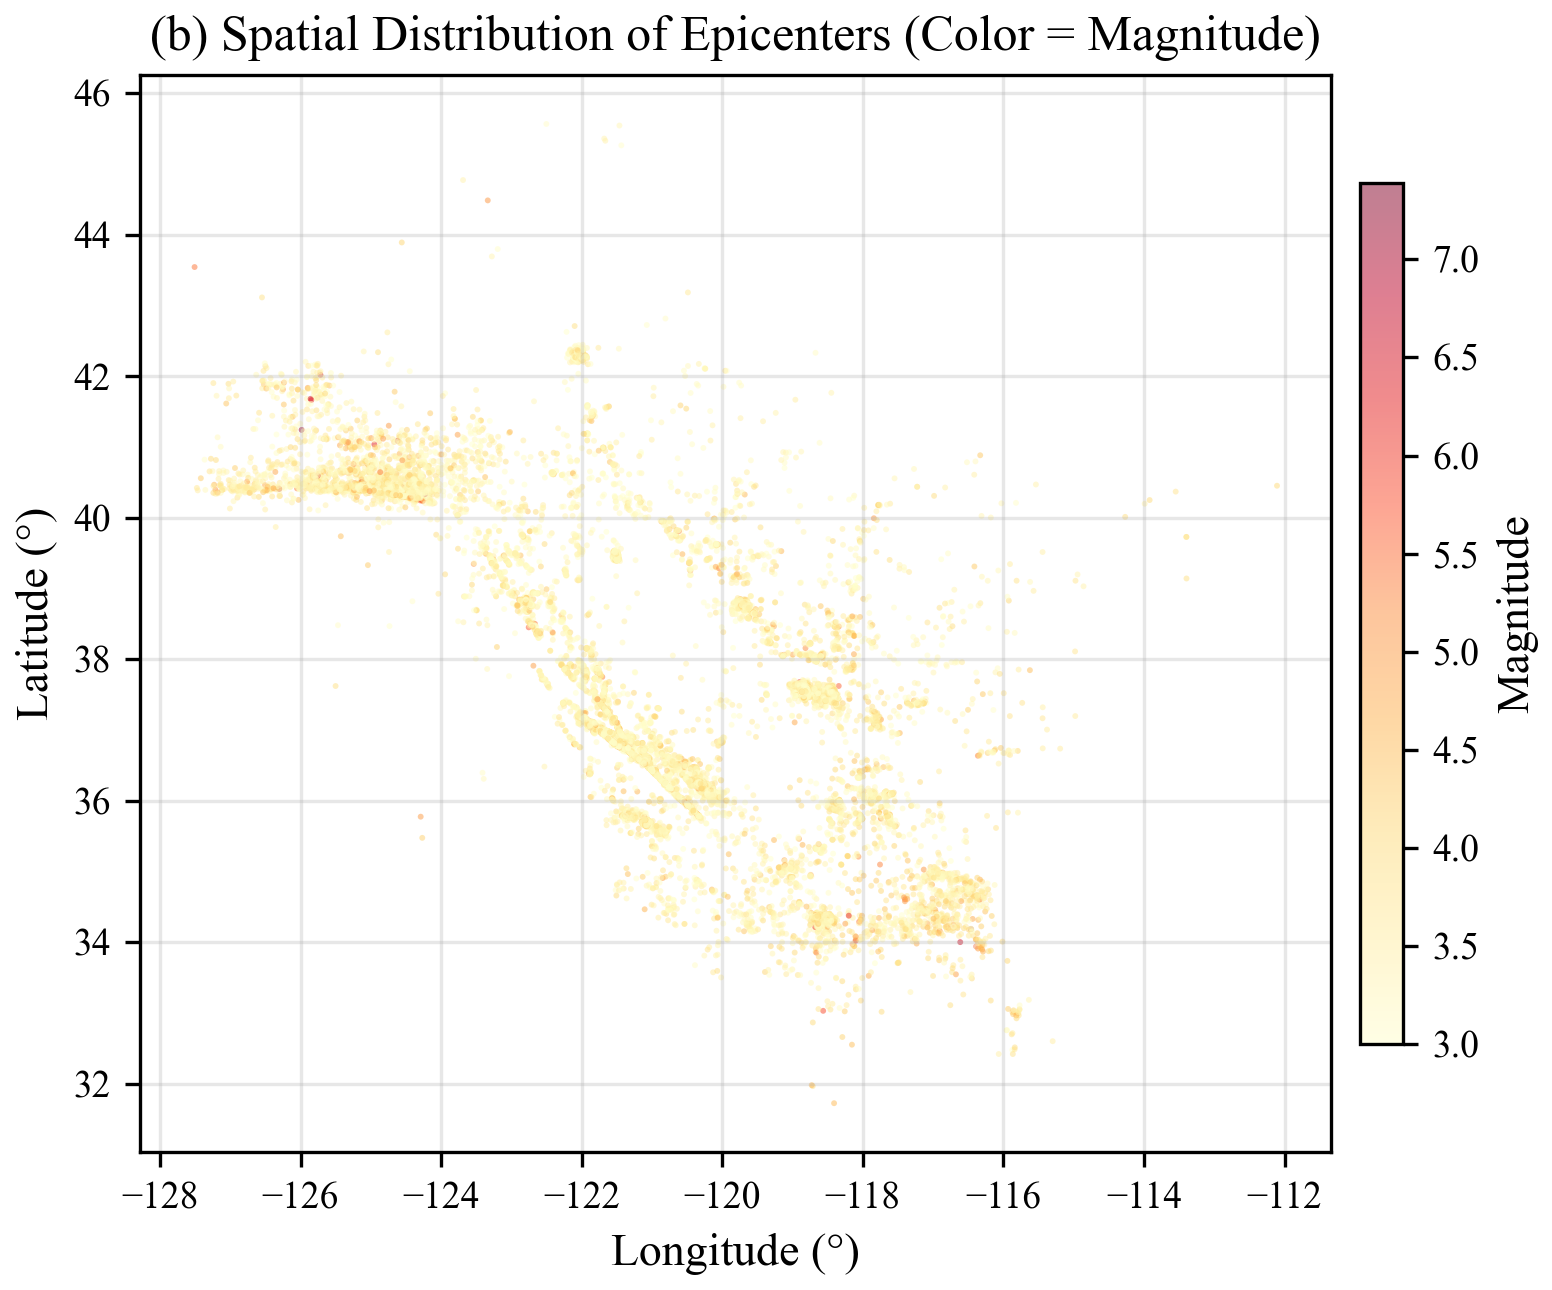
\includegraphics[width=\columnwidth]{fig2_spatial_distribution.png}
\caption{Spatial distribution of 18,030 earthquake epicenters in California, color-coded by magnitude. Clustering is visible along the San Andreas Fault system.}
\label{fig:spatial_dist}
\end{figure}

% ══════════════════════════════════════════════════════════════════════════════
\section{Methodology}
\label{sec:methodology}

\subsection{Feature Engineering}
\label{sec:feature_engineering}

We transform 13 raw columns into 59 ML-ready features organized into five categories (Table~\ref{tab:feature_categories}).

\begin{table}[!t]
\centering
\caption{Feature Engineering Summary (59 Features)}
\label{tab:feature_categories}
\begin{tabular}{@{}lcp{4.2cm}@{}}
\toprule
\textbf{Category} & \textbf{Count} & \textbf{Key Features} \\
\midrule
Temporal & 13 & year, cyclic sin/cos (month, hour, dow), inter-event time \\
Spatial & 8 & lat/lon radians, centroid distance, grid bins \\
Seismological & 10 & log\_depth, stations/gap, close$\times$depth, RMS variants \\
Rolling/Lag & 26 & Rolling mean/std/max (5,10,30), magnitude \& depth lags (1--3), spatial counts \\
Encoded & 2 & Label-encoded magnitude type \\
\bottomrule
\end{tabular}
\end{table}

\textbf{Cyclic encoding.} Periodic variables (month, hour, day-of-week) are encoded as sine–cosine pairs to preserve circular continuity:
\begin{equation}
x_{\sin} = \sin\!\left(\frac{2\pi \cdot x}{P}\right), \quad
x_{\cos} = \cos\!\left(\frac{2\pi \cdot x}{P}\right)
\label{eq:cyclic}
\end{equation}
where $P$ is the period (12 for months, 24 for hours, 7 for days).

\textbf{Rolling statistics.} For windows $w \in \{5, 10, 30\}$, we compute rolling mean, standard deviation, and maximum of past magnitudes and depths:
\begin{equation}
\bar{m}_w(t) = \frac{1}{w} \sum_{i=1}^{w} m_{t-i}
\label{eq:rolling}
\end{equation}
All rolling and lag features use \texttt{shift(1)} to ensure strict temporal causality and prevent data leakage.

\textbf{Leakage prevention.} Magnitude difference features use only lagged values ($m_{t-1} - m_{t-2}$ and $m_{t-2} - m_{t-3}$), never accessing the current target $m_t$.

\subsection{Model Selection}
\label{sec:models}

We evaluate 11 regression algorithms, all wrapped in a \texttt{scikit-learn Pipeline} with \texttt{StandardScaler} preprocessing:

\begin{enumerate}
    \item \textbf{Linear models}: Linear Regression, Ridge ($\alpha=1.0$), Lasso ($\alpha=0.01$), ElasticNet ($\alpha=0.01$, $l_1=0.5$)
    \item \textbf{Tree-based}: Decision Tree ($d_{\max}=15$), Random Forest ($n=100$, $d_{\max}=15$), Extra Trees ($n=100$, $d_{\max}=15$)
    \item \textbf{Boosting}: Gradient Boosting ($n=50$, $d_{\max}=4$), AdaBoost ($n=50$), XGBoost ($n=100$, $d_{\max}=6$)
    \item \textbf{Instance-based}: KNN ($k=7$, distance-weighted)
\end{enumerate}

\subsection{Evaluation Protocol}
\label{sec:evaluation}

Data is split 70/30 (train/test) with temporal ordering preserved. We evaluate using five metrics:

\textbf{Coefficient of Determination ($R^2$):}
\begin{equation}
R^2 = 1 - \frac{\sum_{i=1}^{n}(y_i - \hat{y}_i)^2}{\sum_{i=1}^{n}(y_i - \bar{y})^2}
\label{eq:r2}
\end{equation}

\textbf{Mean Absolute Error (MAE):}
\begin{equation}
\text{MAE} = \frac{1}{n}\sum_{i=1}^{n}|y_i - \hat{y}_i|
\label{eq:mae}
\end{equation}

\textbf{Root Mean Squared Error (RMSE):}
\begin{equation}
\text{RMSE} = \sqrt{\frac{1}{n}\sum_{i=1}^{n}(y_i - \hat{y}_i)^2}
\label{eq:rmse}
\end{equation}

\textbf{Mean Absolute Percentage Error (MAPE):}
\begin{equation}
\text{MAPE} = \frac{100}{n}\sum_{i=1}^{n}\frac{|y_i - \hat{y}_i|}{|y_i|}
\label{eq:mape}
\end{equation}

\textbf{Explained Variance (EV):}
\begin{equation}
\text{EV} = 1 - \frac{\text{Var}(y - \hat{y})}{\text{Var}(y)}
\label{eq:ev}
\end{equation}

\subsection{Hyperparameter Tuning}
\label{sec:tuning}

The top three models from the initial sweep are tuned via \texttt{RandomizedSearchCV} with 20 iterations and 5-fold cross-validation. The search spaces are defined in Table~\ref{tab:hyperparam_space}.

\begin{table}[!t]
\centering
\caption{Hyperparameter Search Spaces}
\label{tab:hyperparam_space}
\begin{tabular}{@{}llp{3.2cm}@{}}
\toprule
\textbf{Model} & \textbf{Parameter} & \textbf{Search Space} \\
\midrule
\multirow{4}{*}{Extra Trees}
& n\_estimators & \{100, 200, 300\} \\
& max\_depth & \{10, 15, 20, 25, None\} \\
& min\_samples\_split & \{2, 5, 10\} \\
& min\_samples\_leaf & \{1, 2, 4\} \\
\midrule
\multirow{4}{*}{XGBoost}
& n\_estimators & \{100, 200, 300\} \\
& max\_depth & \{4, 6, 8, 10\} \\
& learning\_rate & \{0.01, 0.05, 0.1, 0.2\} \\
& subsample & \{0.7, 0.8, 0.9, 1.0\} \\
\midrule
\multirow{4}{*}{\shortstack[l]{Random\\Forest}}
& n\_estimators & \{100, 200, 300\} \\
& max\_depth & \{10, 15, 20, None\} \\
& min\_samples\_split & \{2, 5, 10\} \\
& min\_samples\_leaf & \{1, 2, 4\} \\
\bottomrule
\end{tabular}
\end{table}

The overall pipeline is summarized in Algorithm~\ref{alg:pipeline}.

\begin{algorithm}[!t]
\caption{ML Pipeline for Magnitude Estimation}
\label{alg:pipeline}
\begin{algorithmic}[1]
\REQUIRE Raw CSV with 13 columns, $N = 18{,}030$ events
\ENSURE Trained model, performance reports
\STATE Load and sort data chronologically
\STATE Engineer 59 features (Sec.~\ref{sec:feature_engineering})
\STATE Split: 70\% train ($n = 12{,}618$), 30\% test ($n = 5{,}409$)
\FOR{each of 11 algorithms}
    \STATE Build Pipeline: StandardScaler $\rightarrow$ Estimator
    \STATE Fit on training set
    \STATE Evaluate on test set ($R^2$, MAE, RMSE, MAPE, EV)
\ENDFOR
\STATE Rank models by Test $R^2$
\STATE Select top-$K$ ($K=3$) models
\FOR{each top-$K$ model}
    \STATE RandomizedSearchCV (20 iter, 5-fold CV)
    \STATE Evaluate tuned model on test set
\ENDFOR
\STATE Export best model (\texttt{joblib}), reports (CSV/JSON)
\end{algorithmic}
\end{algorithm}

% ══════════════════════════════════════════════════════════════════════════════
\section{Experimental Results}
\label{sec:results}

\subsection{Initial Model Comparison}

Table~\ref{tab:model_comparison} reports the performance of all 11 models on the 70/30 split. Ensemble methods (XGBoost, Extra Trees, Random Forest) dominate the ranking, while linear models achieve moderate $R^2 \approx 0.16$. The Decision Tree overfits severely (Train $R^2 = 0.72$, Test $R^2 = -0.18$), and KNN shows complete memorization (Train $R^2 = 1.0$, Test $R^2 = 0.04$).

\begin{table*}[!t]
\centering
\caption{Performance Comparison of 11 Regression Models (70/30 Split, No CV)}
\label{tab:model_comparison}
\begin{tabular}{@{}rlcccccr@{}}
\toprule
\textbf{Rank} & \textbf{Model} & \textbf{Train $R^2$} & \textbf{Test $R^2$} & \textbf{MAE} & \textbf{RMSE} & \textbf{MAPE (\%)} & \textbf{Time (s)} \\
\midrule
1 & XGBoost               & 0.6268 & \textbf{0.3281} & 0.2540 & 0.3467 & 7.18 & 0.5 \\
2 & Extra Trees            & 0.7467 & 0.3154 & 0.2565 & 0.3500 & 7.25 & 1.3 \\
3 & Random Forest          & 0.7263 & 0.3113 & 0.2563 & 0.3510 & 7.24 & 7.2 \\
4 & Gradient Boosting      & 0.3659 & 0.2873 & 0.2643 & 0.3571 & 7.46 & 11.2 \\
5 & Ridge Regression       & 0.1632 & 0.1659 & 0.2880 & 0.3863 & 8.15 & 0.01 \\
6 & Linear Regression      & 0.1632 & 0.1659 & 0.2880 & 0.3863 & 8.15 & 0.02 \\
7 & ElasticNet             & 0.1540 & 0.1612 & 0.2897 & 0.3874 & 8.19 & 0.02 \\
8 & Lasso Regression       & 0.1449 & 0.1512 & 0.2919 & 0.3897 & 8.25 & 0.01 \\
9 & KNN Regressor          & 1.0000 & 0.0389 & 0.3040 & 0.4146 & 8.55 & 0.01 \\
10 & AdaBoost              & 0.0736 & 0.0264 & 0.3375 & 0.4173 & 9.84 & 7.7 \\
11 & Decision Tree          & 0.7158 & $-$0.1770 & 0.3083 & 0.4589 & 8.66 & 0.8 \\
\bottomrule
\end{tabular}
\end{table*}

Fig.~\ref{fig:model_comparison} visualizes the test $R^2$ for all models, and Fig.~\ref{fig:radar} presents a radar chart of the top five models across multiple metrics.

\begin{figure}[!t]
\centering
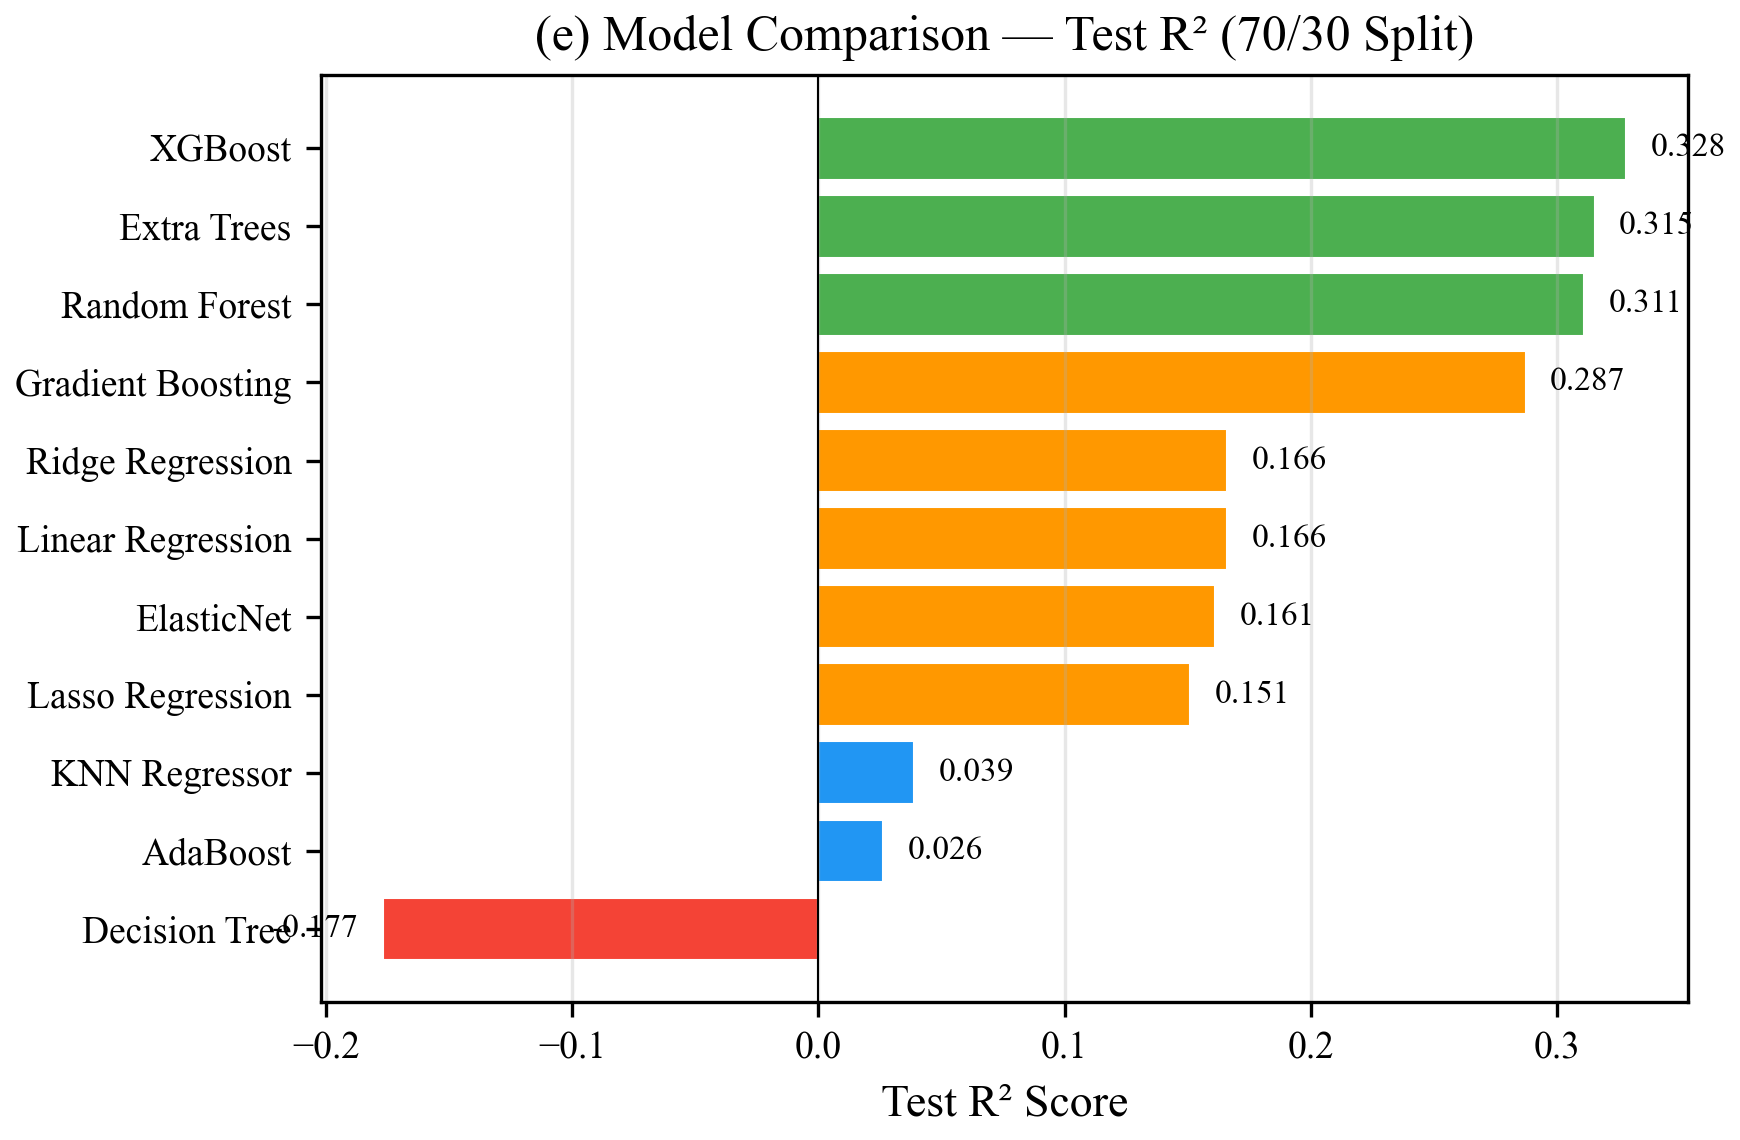
\includegraphics[width=\columnwidth]{fig5_model_comparison.png}
\caption{Test $R^2$ scores for all 11 regression models. Ensemble methods (XGBoost, Extra Trees, Random Forest) substantially outperform linear baselines.}
\label{fig:model_comparison}
\end{figure}

\begin{figure}[!t]
\centering
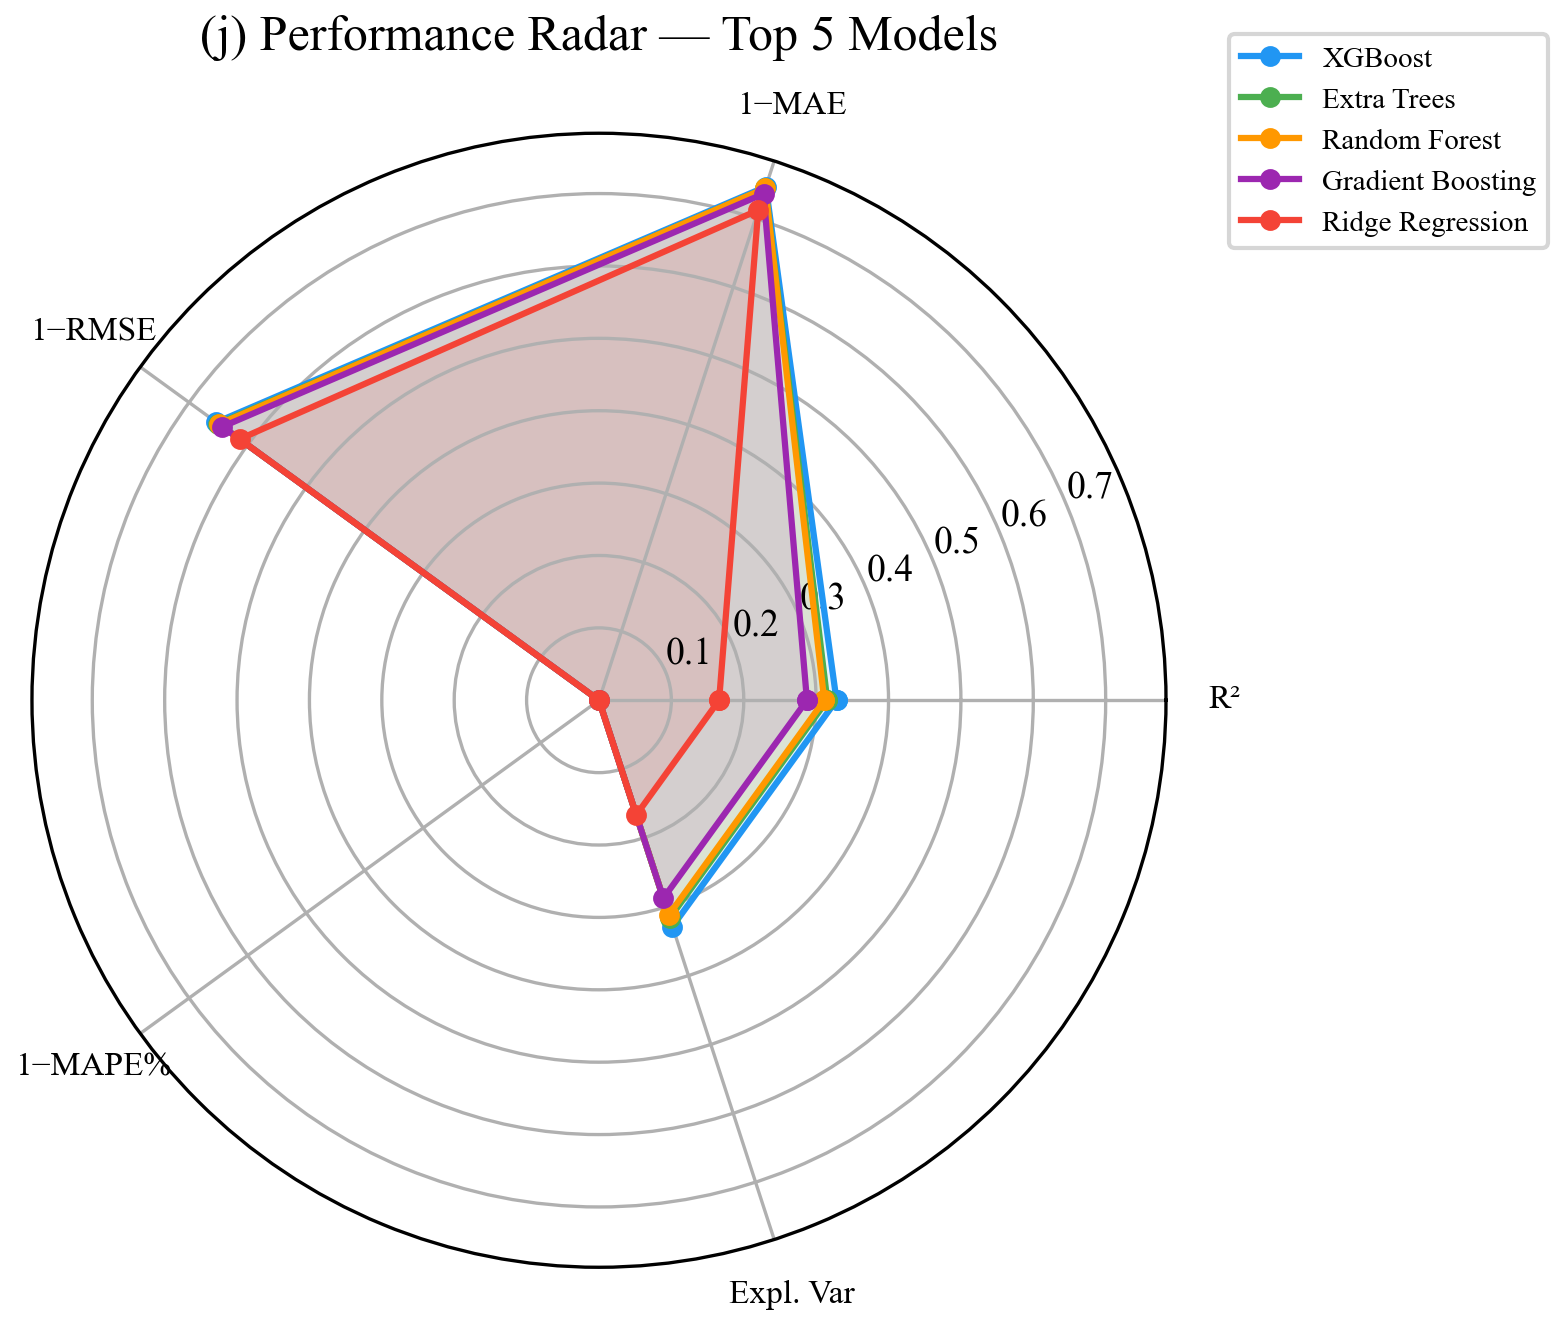
\includegraphics[width=\columnwidth]{fig10_metric_radar.png}
\caption{Radar chart comparing top 5 models across five metrics (higher is better; error metrics inverted).}
\label{fig:radar}
\end{figure}

\subsection{Hyperparameter Tuning Results}

Table~\ref{tab:tuning_results} compares the tuned models against their initial versions. The tuned Extra Trees achieves the highest overall performance, surpassing the initially top-ranked XGBoost.

\begin{table}[!t]
\centering
\caption{Tuned vs. Initial Model Performance}
\label{tab:tuning_results}
\begin{tabular}{@{}lcccc@{}}
\toprule
\textbf{Model} & \textbf{$R^2$} & \textbf{MAE} & \textbf{RMSE} & \textbf{CV $R^2$} \\
\midrule
Extra Trees (tuned)    & \textbf{0.3297} & \textbf{0.2522} & \textbf{0.3463} & 0.3037 \\
XGBoost (tuned)        & 0.3286 & 0.2547 & 0.3466 & 0.2960 \\
XGBoost (initial)      & 0.3281 & 0.2540 & 0.3467 & --- \\
Random Forest (tuned)  & 0.3158 & 0.2554 & 0.3499 & 0.2929 \\
\bottomrule
\end{tabular}
\end{table}

The optimal Extra Trees hyperparameters are: \texttt{n\_estimators}$=300$, \texttt{max\_depth}$=20$, \texttt{min\_samples\_split}$=5$, \texttt{min\_samples\_leaf}$=4$. The modest gap between CV $R^2$ (0.3037) and test $R^2$ (0.3297) suggests minimal overfitting.

Fig.~\ref{fig:tuned_vs_initial} provides a visual comparison of $R^2$, MAE, and RMSE across tuned and initial model variants.

\begin{figure}[!t]
\centering
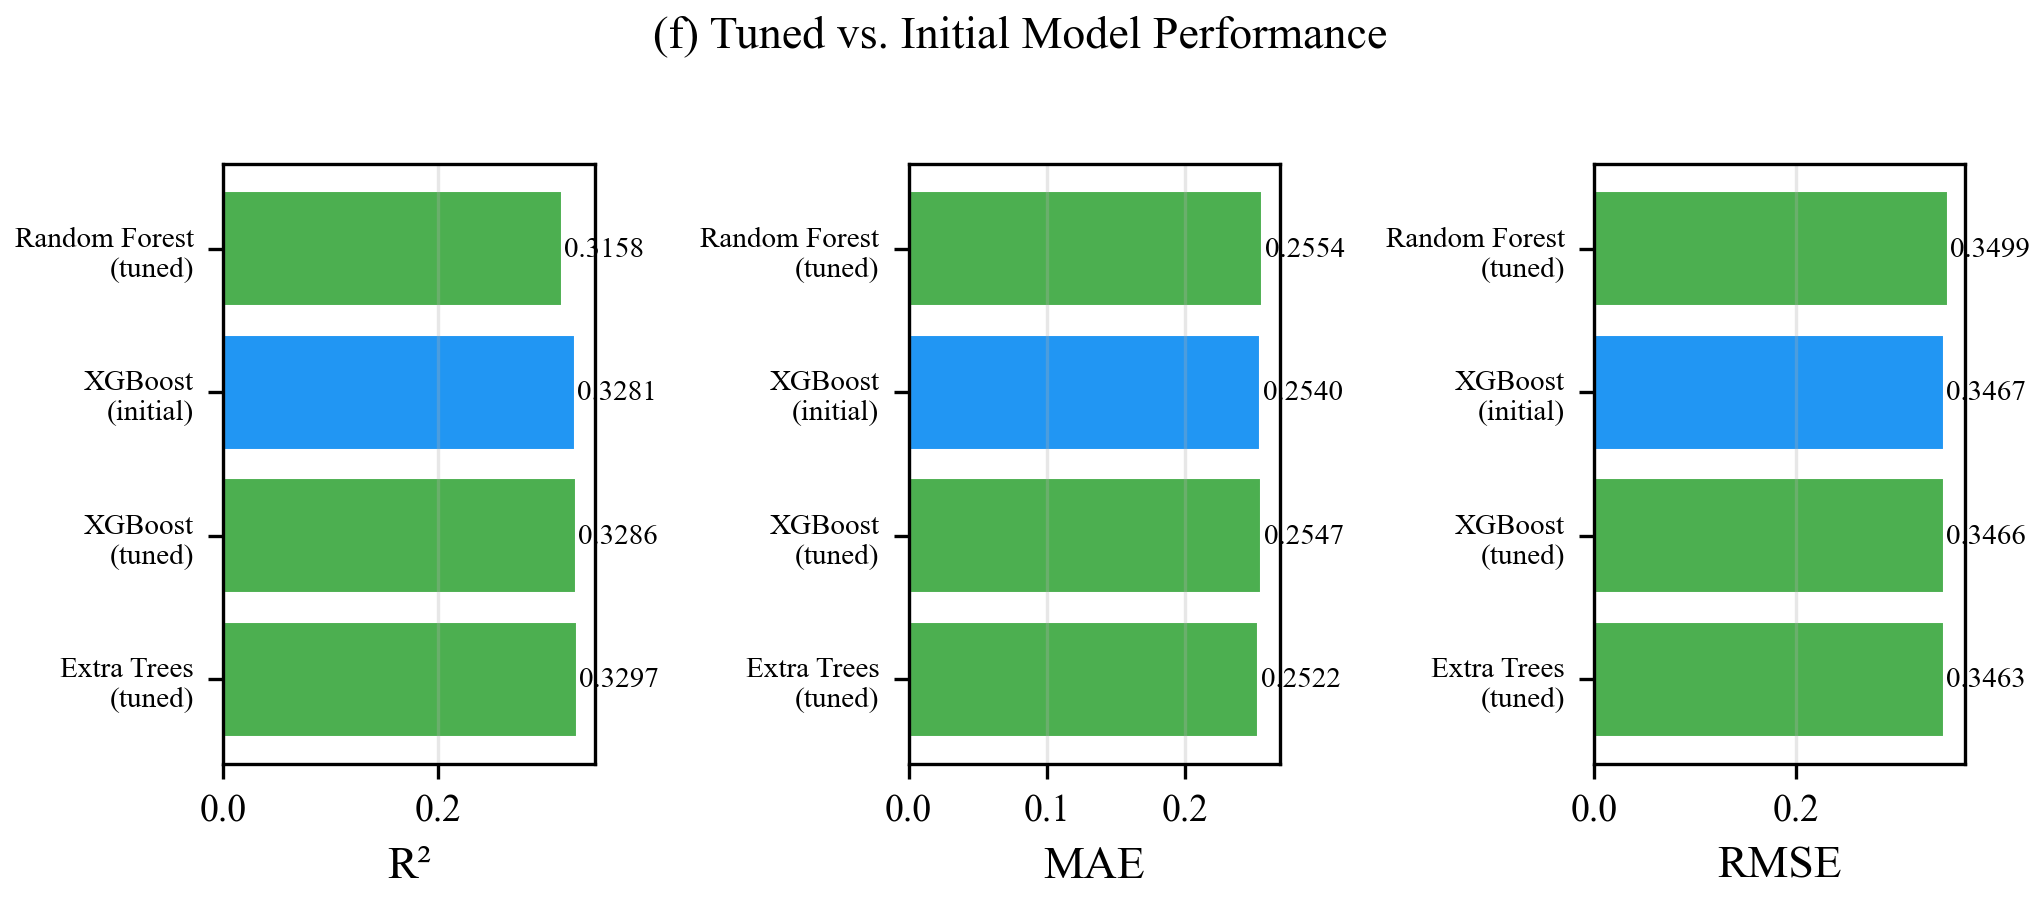
\includegraphics[width=\columnwidth]{fig6_tuned_vs_initial.png}
\caption{Three-metric comparison of tuned vs.\ initial model variants.}
\label{fig:tuned_vs_initial}
\end{figure}

\subsection{Feature Importance Analysis}

Fig.~\ref{fig:feat_imp} shows the top 20 features by Gini importance from the tuned Extra Trees model. The most informative feature is \texttt{No\_of\_Stations} (11.98\%), followed by \texttt{Magnitude\_type\_enc} (8.66\%) and \texttt{year} (4.93\%).

\begin{figure}[!t]
\centering
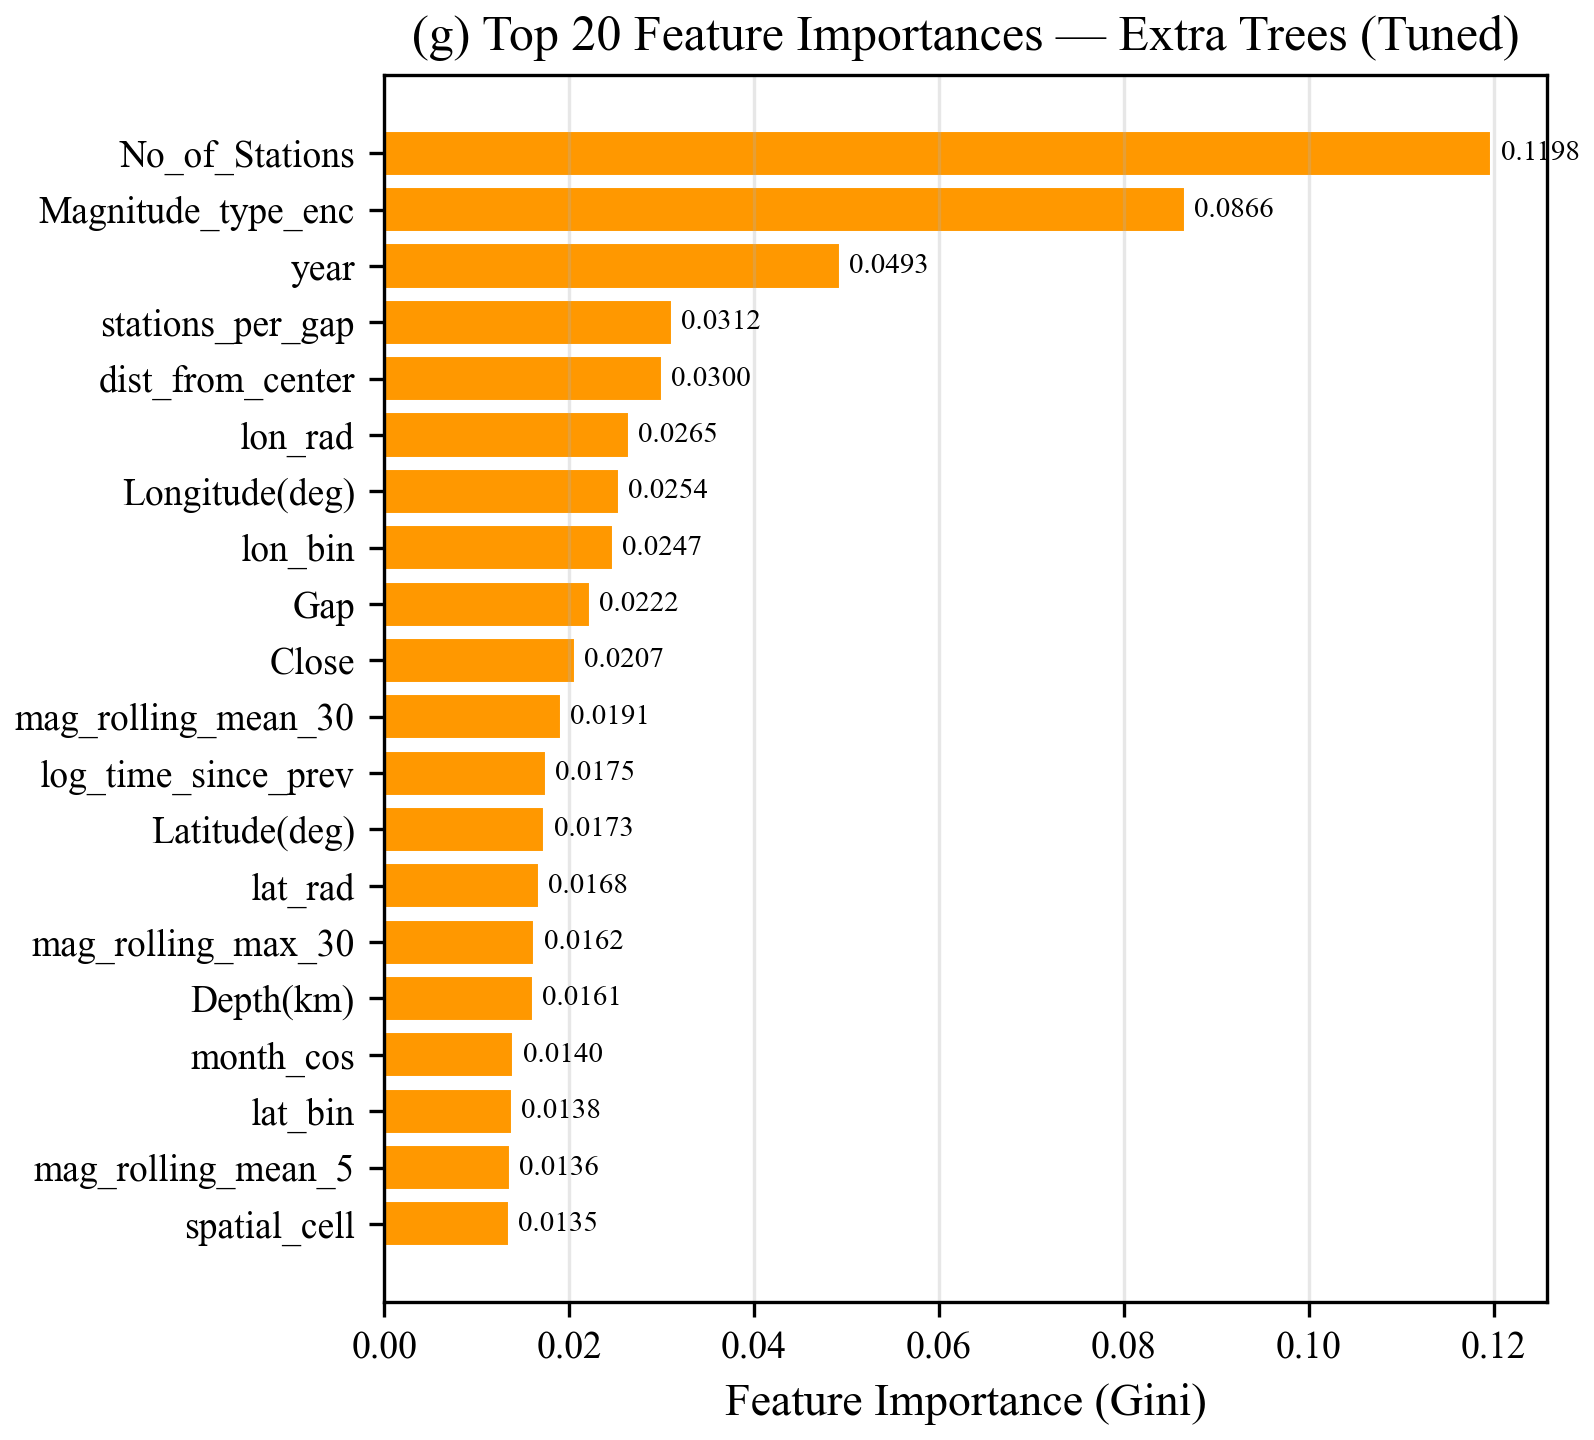
\includegraphics[width=\columnwidth]{fig7_feature_importance.png}
\caption{Top 20 feature importances from the tuned Extra Trees Regressor (Gini impurity).}
\label{fig:feat_imp}
\end{figure}

Fig.~\ref{fig:feat_cats} aggregates importance by feature category. Rolling/lag statistics contribute 26.1\% of total importance, followed by seismological features (24.8\%), spatial (15.3\%), temporal (14.2\%), and encoded variables (8.7\%).

\begin{figure}[!t]
\centering
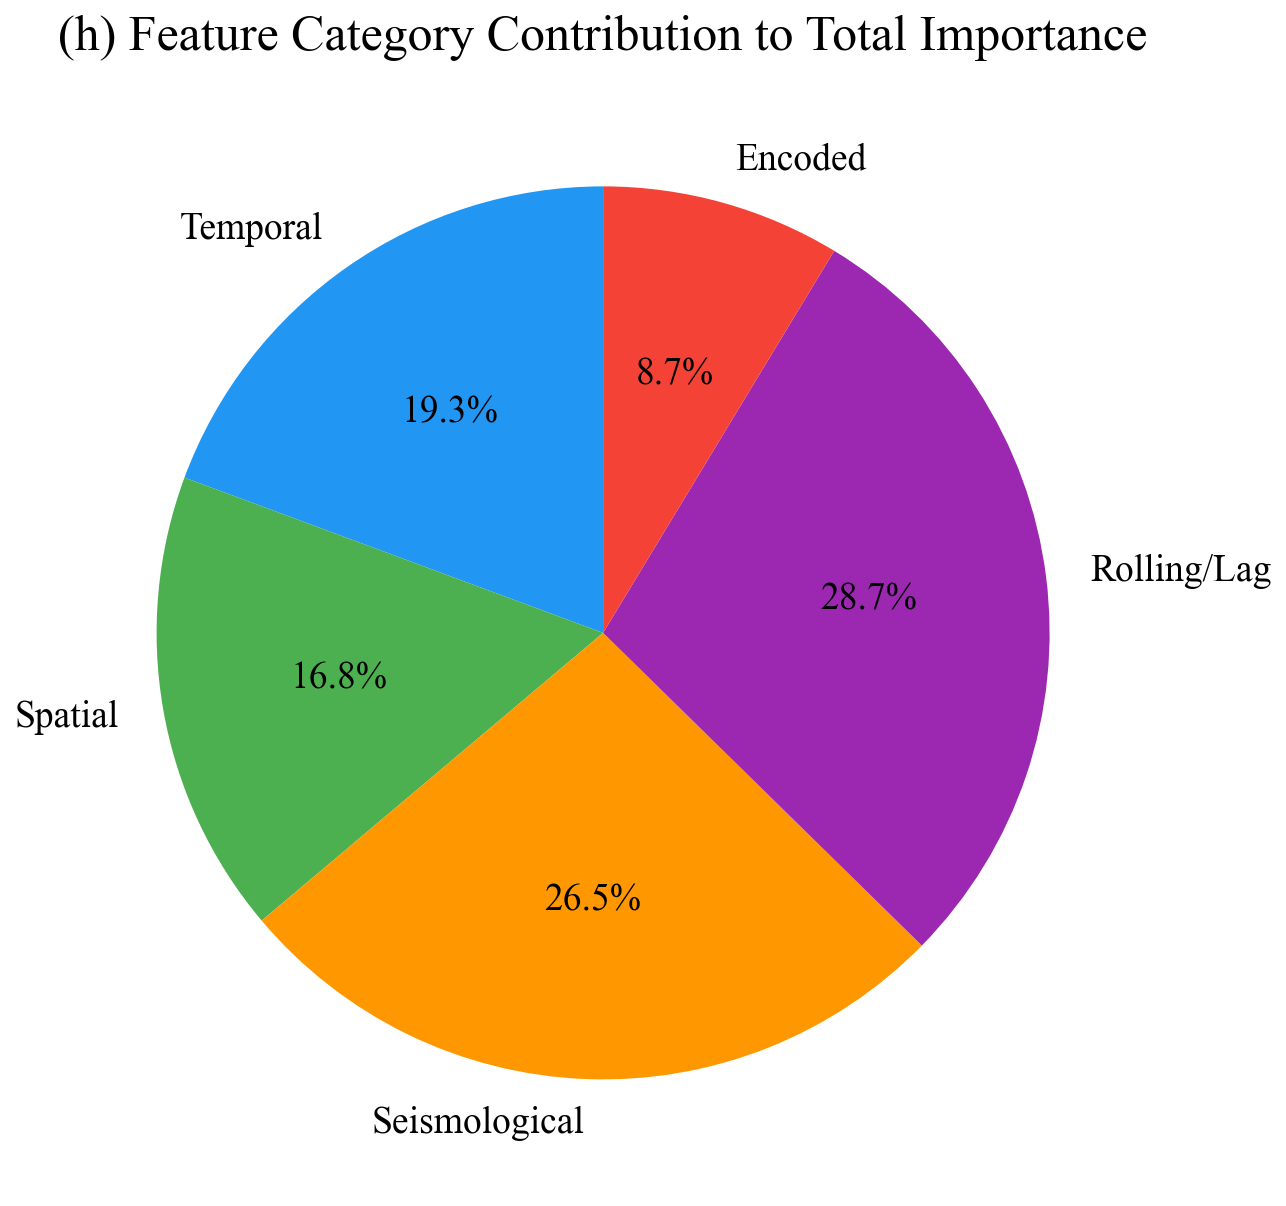
\includegraphics[width=\columnwidth]{fig8_feature_categories.png}
\caption{Aggregated feature importances by category.}
\label{fig:feat_cats}
\end{figure}

\subsection{Data Exploration}

The correlation heatmap (Fig.~\ref{fig:correlation}) reveals weak correlations between raw features and magnitude, with \texttt{No\_of\_Stations} showing the strongest linear association ($r \approx 0.35$). This weak linearity motivates the use of nonlinear ensemble methods.

\begin{figure}[!t]
\centering
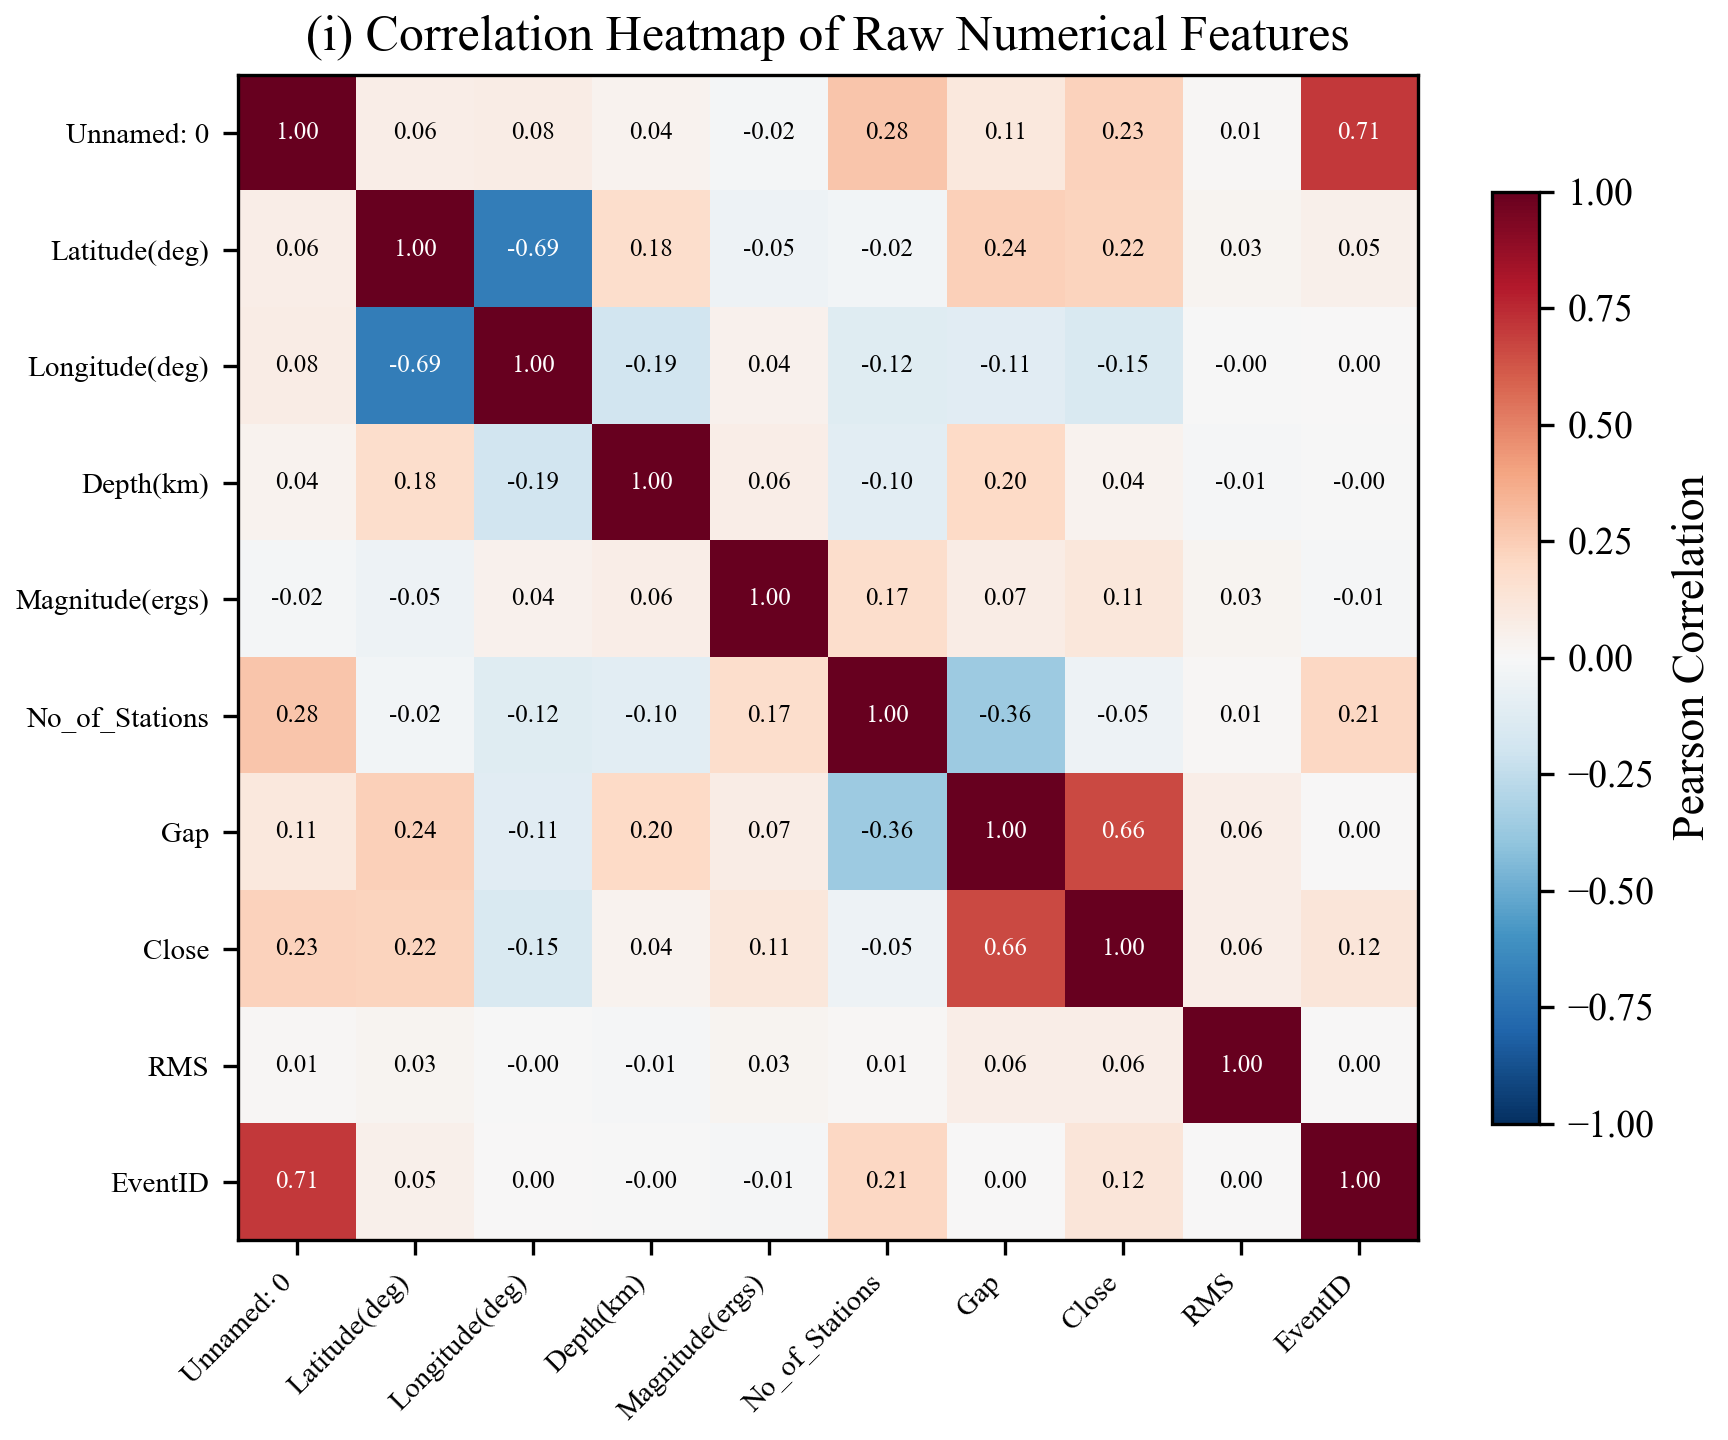
\includegraphics[width=\columnwidth]{fig9_correlation_heatmap.png}
\caption{Pearson correlation heatmap of raw numerical features. Weak correlations with the target motivate nonlinear modeling.}
\label{fig:correlation}
\end{figure}

Fig.~\ref{fig:depth_mag} shows the relationship between hypocentral depth and magnitude. Most events concentrate at shallow depths ($<$20~km) with no strong depth-magnitude trend, consistent with California's predominantly shallow seismicity.

\begin{figure}[!t]
\centering
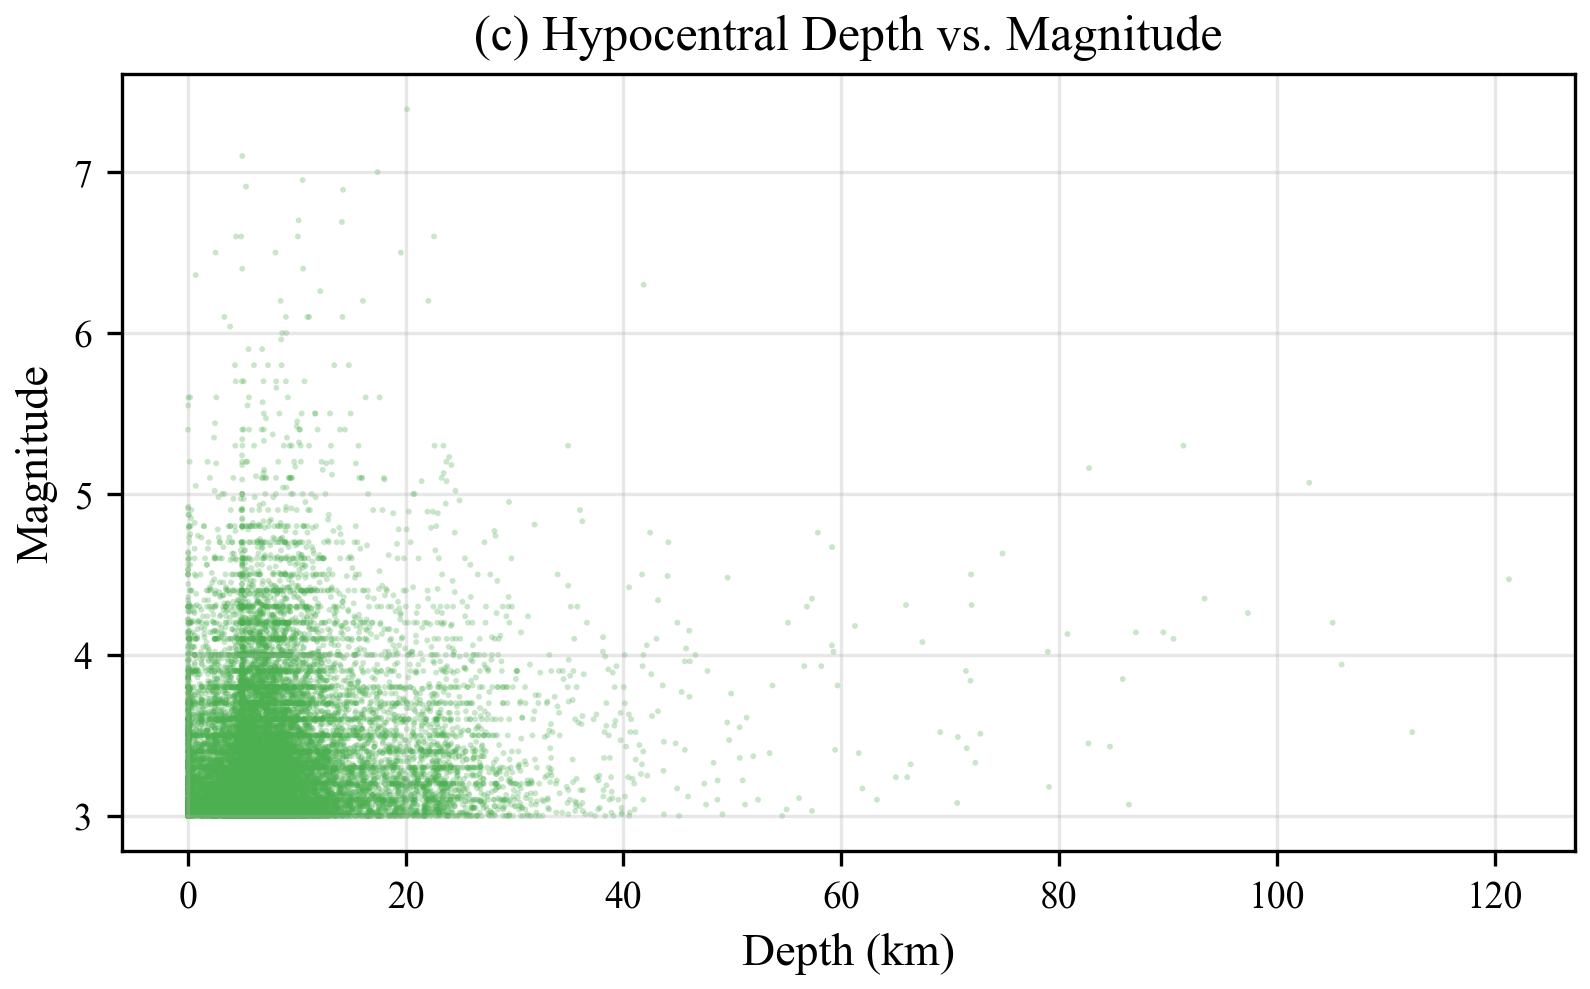
\includegraphics[width=\columnwidth]{fig3_depth_vs_magnitude.png}
\caption{Hypocentral depth vs.\ magnitude. Most events are shallow ($<$20~km) with no clear trend.}
\label{fig:depth_mag}
\end{figure}

Fig.~\ref{fig:temporal} displays the annual frequency of events and mean magnitude over the 41-year observation period.

\begin{figure}[!t]
\centering
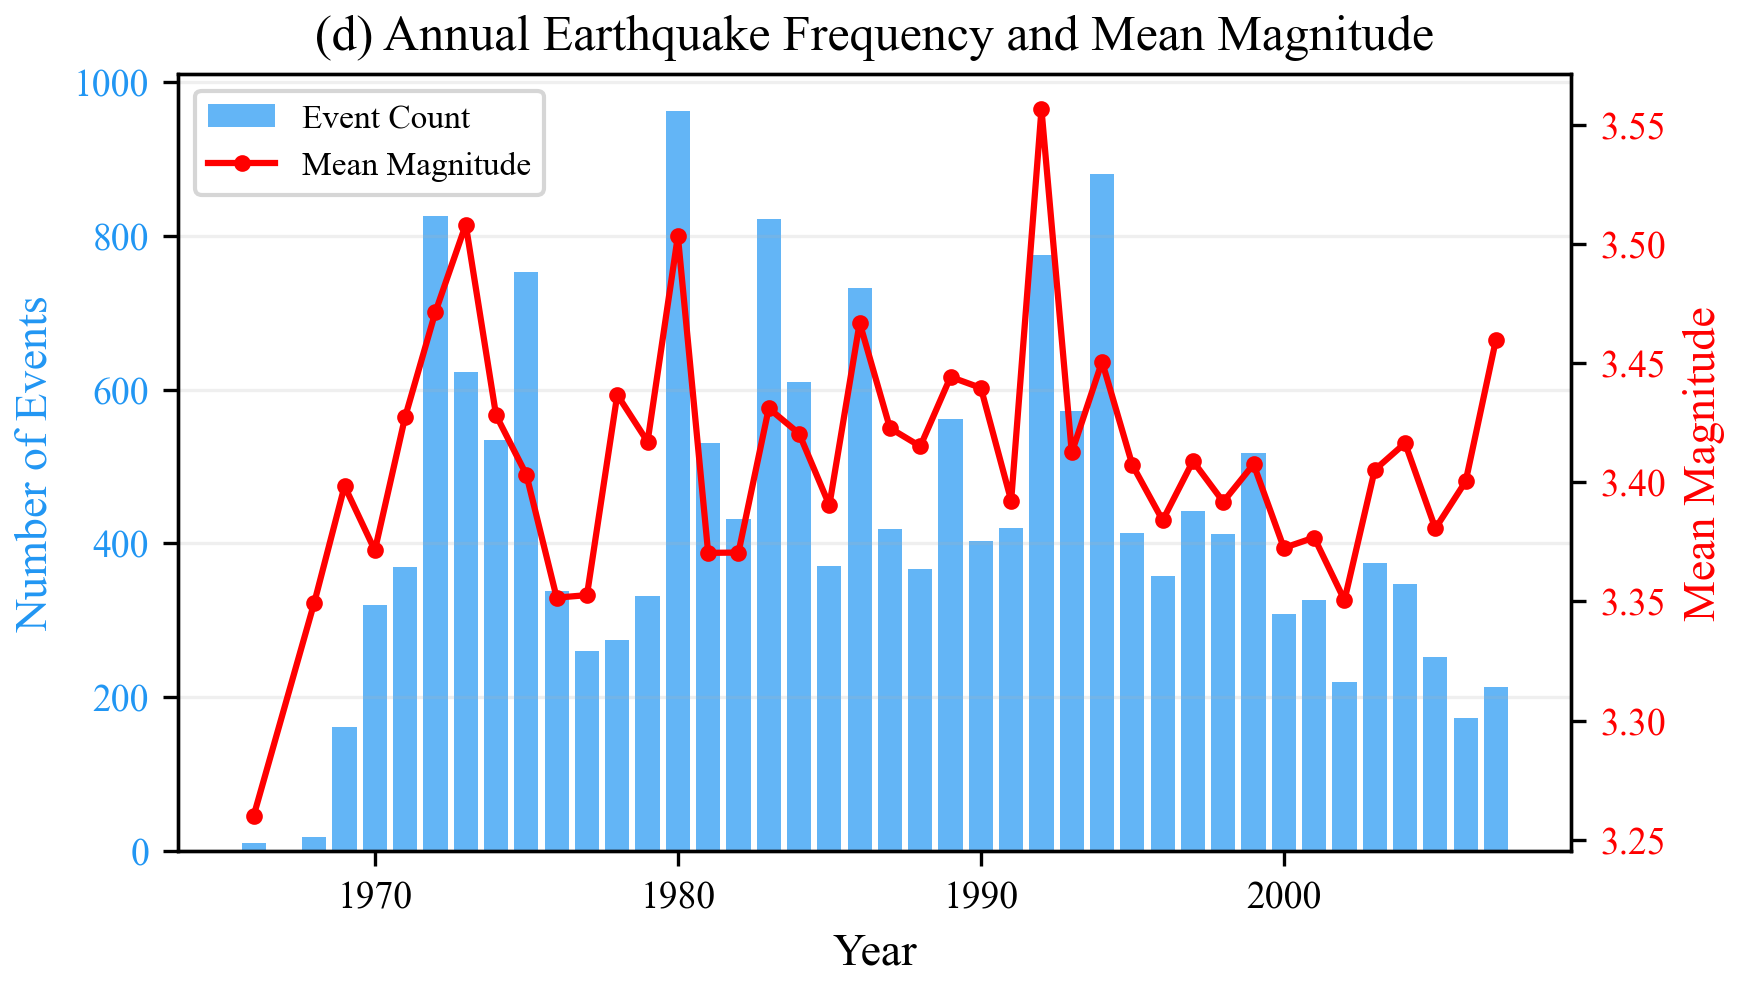
\includegraphics[width=\columnwidth]{fig4_temporal_distribution.png}
\caption{Annual earthquake frequency (bars) and mean magnitude (line) from 1966 to 2007.}
\label{fig:temporal}
\end{figure}

% ══════════════════════════════════════════════════════════════════════════════
\section{Discussion}
\label{sec:discussion}

\subsection{Interpretation of Results}

The best model achieves $R^2 = 0.3297$, meaning it explains approximately 33\% of the variance in earthquake magnitudes. While this may appear modest compared to many ML benchmarks, it is consistent with the fundamental nature of the problem:

\begin{itemize}
    \item Earthquake magnitude is governed by rupture dynamics and stress-state variables that are not observable from surface catalog data alone \cite{geller1997}.
    \item The Gutenberg-Richter distribution implies that magnitude is largely controlled by self-organized criticality, introducing irreducible stochasticity \cite{turcotte1997}.
    \item An MAE of 0.25 magnitude units represents practical utility for relative magnitude assessment within a network.
\end{itemize}

\subsection{Station Count as Top Predictor}

The dominance of \texttt{No\_of\_Stations} (12\%) aligns with seismological understanding: larger earthquakes generate more detectable arrivals across a wider network, while smaller events may only be recorded by nearby stations. This feature captures both the true physical signal and an observational bias inherent to seismic network geometry.

\subsection{Ensemble Superiority}

Tree-based ensembles outperform linear models by a factor of $\sim$2$\times$ in $R^2$, confirming the presence of nonlinear interaction effects in the feature space. The Extra Trees randomized splitting strategy provides additional regularization compared to Random Forest's greedy splits, yielding marginally better generalization.

\subsection{Overfitting Patterns}

The Decision Tree and KNN models exhibit classic overfitting: near-perfect training scores with poor test performance. The Decision Tree's unrestricted depth memorizes training noise, while KNN's distance-based lookup fails in the 59-dimensional feature space due to the curse of dimensionality.

\subsection{Limitations}

\begin{enumerate}
    \item \textbf{Geographic scope}: The model is trained exclusively on California seismicity and may not generalize to other tectonic settings.
    \item \textbf{Temporal range}: Data from 1966--2007 may not capture recent changes in network instrumentation or seismicity patterns.
    \item \textbf{Feature availability}: Several features (station count, gap, RMS) require processed seismological data not available in real-time early warning scenarios.
    \item \textbf{Target distribution}: The narrow magnitude range (3.0--7.39) with strong skew toward $M \approx 3.0$ limits the model's ability to distinguish large events.
    \item \textbf{Irreducible error}: The inherent stochasticity of earthquake processes places a fundamental ceiling on achievable $R^2$ from catalog features alone.
\end{enumerate}

\subsection{Ethical Considerations}

This work is presented strictly as a \emph{research tool}, not a prediction system. Earthquake prediction—specifying the time, location, and magnitude of future events—remains scientifically impossible with current technology \cite{geller1997}. Any deployment of magnitude estimation models must include prominent disclaimers and should never be used for evacuation decisions or public safety advisories without expert oversight.

% ══════════════════════════════════════════════════════════════════════════════
\section{Conclusion}
\label{sec:conclusion}

We have presented a comprehensive machine learning pipeline for earthquake magnitude estimation using 59 engineered features and 11 regression algorithms evaluated on 18,030 NCSN catalog events. The tuned Extra Trees Regressor achieves the best performance ($R^2 = 0.3297$, MAE $= 0.2522$), demonstrating that ensemble methods with carefully engineered spatiotemporal features can extract meaningful predictive signal from seismic catalog data.

Future work could explore: (a) waveform-level deep learning features to complement catalog metadata, (b) region-transfer learning to adapt the model to non-California tectonic settings, (c) probabilistic regression to provide calibrated uncertainty estimates, and (d) integration with real-time seismic data streams for operational applications.

The complete pipeline, trained model, and interactive visualization tool are available at: \url{https://github.com/ariktheone/earthquake-prediction}.

% ══════════════════════════════════════════════════════════════════════════════
\section*{Reproducibility}

All code, data, and trained models are open-source under the MIT License. The ML pipeline can be re-executed via:
\begin{verbatim}
cd model_prep && python run_pipeline.py
\end{verbatim}
Total pipeline runtime is approximately 28 minutes on a standard workstation.

% ══════════════════════════════════════════════════════════════════════════════
\section*{Acknowledgments}
The authors thank the Northern California Earthquake Data Center (NCEDC) and the USGS for providing open-access seismic catalog data.

% ══════════════════════════════════════════════════════════════════════════════
\balance
\begin{thebibliography}{10}

\bibitem{geller1997}
R.~J. Geller, ``Earthquake prediction: A critical review,'' \emph{Geophysical Journal International}, vol.~131, no.~3, pp.~425--450, 1997.

\bibitem{kanamori1977}
H.~Kanamori, ``The energy release in great earthquakes,'' \emph{Journal of Geophysical Research}, vol.~82, no.~20, pp.~2981--2987, 1977.

\bibitem{mousavi2020}
S.~M. Mousavi, W.~Zhu, Y.~Sheng, and G.~C. Beroza, ``CRED: A deep residual network of convolutional and recurrent units for earthquake signal detection,'' \emph{Scientific Reports}, vol.~9, no.~1, p.~10267, 2019.

\bibitem{derakhshani2013}
R.~Derakhshani and M.~Tavallaie, ``Predicting earthquake magnitude using artificial neural networks and support vector regression,'' \emph{Journal of Sciences, Islamic Republic of Iran}, vol.~24, no.~3, pp.~249--264, 2013.

\bibitem{perol2018}
T.~Perol, M.~Gharbi, and M.~Denolle, ``Convolutional neural network for earthquake detection and location,'' \emph{Science Advances}, vol.~4, no.~2, p.~e1700578, 2018.

\bibitem{asim2018}
K.~M. Asim, F.~Martinez-Alvarez, A.~Basit, and T.~Iqbal, ``Earthquake magnitude prediction in Hindukush region using machine learning techniques,'' \emph{Natural Hazards}, vol.~85, no.~1, pp.~471--486, 2017.

\bibitem{bergen2019}
K.~J. Bergen, P.~A. Johnson, M.~V. de~Hoop, and G.~C. Beroza, ``Machine learning for data-driven discovery in solid earth geoscience,'' \emph{Science}, vol.~363, no.~6433, p.~eaau0323, 2019.

\bibitem{turcotte1997}
D.~L. Turcotte, \emph{Fractals and Chaos in Geology and Geophysics}, 2nd~ed.\hskip 1em plus 0.5em minus 0.4em Cambridge University Press, 1997.

\bibitem{ncedc}
Northern California Earthquake Data Center (NCEDC), ``NCSN earthquake catalog,'' \url{https://ncedc.org/}, accessed: 2026.

\bibitem{hough2010}
S.~E. Hough, \emph{Predicting the Unpredictable: The Tumultuous Science of Earthquake Prediction}.\hskip 1em plus 0.5em minus 0.4em Princeton University Press, 2010.

\end{thebibliography}

\end{document}
